%!TEX TS-program = xelatex
%!TEX encoding = UTF-8 Unicode
% !TEX root = ../../metp.tex

\begin{refsection}

\section{RIVERBERI}
\thispagestyle{empty}

Nonostante l'acustica architettonica sia stata per millenni parte integrante
della progettazione di strutture, la materia ha ottenuto una base
scientifica solida solo ai primi del novecento per opera di \ws. \cite{ws:rev}
La definizione del tempo di riverbero da parte di Sabine è il punto di partenza
anche nella letteratura sulla modellazione digitale dell'effetto ad opera di
\ms. \cite{ms:rev62, ms:rev64} Dopo Sabine il tempo di riverbero può essere
descritto, misurato, previsto. Tutto quello che sappiamo fare oggi continua ad
attingere alle sue ricerce.

\subsection{Sabine}

\begin{quote}
  The following investigation was not undertaken at first by choice, but devolved
  on the writer in 1895, through instructionns from the Corporation of Harvard
  University to propose changes from remedying the acoustical difficulties in
  the lecture-room o the Fogg Art Museum, a building that had just been completed.
  About two years were spent in experimenting on this room, and permanet changes
  where then made. Almost immediately afterward it become certain that a new
  Boston Music Hall would be erected, and the questions arising in the
  consideration of its plans forced a not unwelcome continuance of the general
  investigation. \cite{ws:rev}
\end{quote}

Trovo significativo che una ricerca così approfondita e miliare possa essere
scaturita da una semplice problematica come quella di dover analizzare e
correggere l'acustica di una sala universitaria. Sulla base di un vuoto letterario,
nulla di organico sul fenomeno del riverbero se non per cenni sparsi provenienti
dalla storia della fisica, \ms~ ha costruito una ricerca organica, con seri
problemi da risolvere, anche di diversa natura, come per esempio la scelta del
cronografo (1985) per misurare il tempo

\begin{quote}
  \ldots perfect noiselessnness, portability, and capacity to measure intervals
  of time from a half of second to ten seconds with considerable accuracy. \cite{ws:rev}
\end{quote}

Sono proprio queste parole a rivelare che non poteva essereci un momento diverso
nella storia dell'uomo in cui la convergenza di esigenze e possibilità tecniche
avrebbe portato alla soluzione di problematiche irrisolte per secoli.

\begin{quote}
  In order that hearing may be good in any auditorium, it is necessary that the
  sound should be sufficiently loud; that the simultaneous components of a
  complex sound should maintain their proper relative intensities;
  and that the successive sounds in rapidly moving articulation, either of speech
  or music, should be clear and distinct, free from each other and from extraneous
  noises. Thesethree are the necessary, as they are the entirely sufficient,
  conditions for good hearing. \cite{ws:rev}
\end{quote}

Una tripletta di problemi minimi da comprendere e risolvere per rendere accettabile
il riverbero acustico di un ambiente.

\subsubsection{Loudness}

Illustrando una condizione semplice di auditorium in forma di spazio piano,
con un oratore ed un ascoltatore, \ws~ introduce il concetto di propagazione
del suono in forma emisferica, che si riduce di intensità all'aumentare della
sua dimensione (distanza dall'origine) proporzionalmente. Aumenta il pubblico,
il suono perde intensità più rapidamente, assorbito. La parte superiore della
propagazione si muove libera, non affetta da assorbimenti. I primi accorgimenti:
elevare l'oratore ed alzare da terra le file posteriori: il teatro Greco. Un tetto
su questa struttura incrementerebbe l'intensità media, soprattutto dei suoni
sostenuti nel tempo, e ne bilancerebbe la resa tra fronte e fondo sala.

\begin{quote}
  The problem of calculating the loudness at different parts of such an
  auditorium is, obviously, complex, but it is perfectly determinate, and as
  soon as the reflecting and absorbing power of the audience and of the various
  wall-surfaces are known it can be solved approximately. \cite{ws:rev}
\end{quote}

Ne ricaviamo la prima ufficiale considerazione: non si può parlare di Riverbero,
al singolare, ma di Riverberi di un luogo. Perfettamente determinati, calcolabili,
ma molti per ogni ambiente che descriviamo.

\subsubsection{Distortion of Complex Sounds: Interference and Resonance}

In termini di \emph{loudness}, i suoni diretti ed i suoni riflessi si rinforzano
l'un laltro quando viaggiano insieme. Possono però trovarsi nella condizione di
cancellarsi a vicenda. Nella descrizione del ronte d'onda che si muove per
successioni di stati opposti, compressioni e rarefazioni, si possono avere
condizioni in cui il suono riflesso da pareti distinte produca nello spazio della
sala una zona di incontro di queste riflessioni, in cui entrambe le compressioni e
le rarefazioni si trovino rinforzate, in fase. Ma si può avere l'occorrenza opposta,
un punto di incontro in cui le compressioni e le rarefazioni non si succedono ma
si sovrappongono, annullandosi. Tutto questo accade in relazione al suono emesso,
alla sua altezza, che variando, varia l'intero stato di equilibrio, l'inntero stato
di interferenza.

C'è un altro fenomeno che occorre in queste circostanze, in relazione con
l'intererenza, ovvero la risonanza.

\begin{quote}
  The word \emph{resonance} has been used loosely as synonymous with
  \emph{reverberation}, and even with \emph{echo}, and is so given in some of
  the more voluminous but less exact popular dictionaries. In scientific
  literature the term has received a very definite and precise application to
  the phenomenon, wherever it may occur, of the growth of a vibratory motion of
  an elastic body under periodic force stimed to its natural rates of vibration.
  A word having this significance is necessary; and it is very desirable that
  the term should not, even popularly, by meaning many things, cease to mean
  anything exactly. \cite{ws:rev}
\end{quote}

Gli uomini che chiedono rispetto per le parole, meritano rispetto, perché
rispettano gli uomini. Anche questa è risonanza.

\subsubsection{Confusion: Reverberation, Echo and Extraneus Sounds}

Si entra così nel cuore della ricerca di \ws, l'atto pratico di comprendere il
malfunzionamento acustico del luogo speciico, cinque secondi ed oltre di riverbero
tale da rendere impossibile comprendere la propria voce in una semplice discussione.
Il fenomeno definito \rev~ il processo delle rilessioni multiple,
tra superfici, pareti, soffitto e pavimento, dapprima da una e poi da un'altra e
poi da molte superici, cambiando (o perdendo) un poco ad ogni rilessione, fino
a diventare inudibile. Questo il fenomeno \rev, che include il caso
speciale denominato \eco. Il \rev~ consiste inoltre in una massa
di suono che riempie uno spazio della quale è impossibile cogliere ed analizzare
la singola riflessione. Il termine \eco~ è riservato al caso specifico di
riflessione pulita, singola, generata da una singola superficie ed a volte ripetuta,
nel caso di più superfici riflettenti. Nel \rev~ ci concentriamo a definirne il
tasso di decadimento del suono nel tempo, nel caso dell'\eco~ l'intensità è un
afttore secondario, mentre risulta un fattore discriminante l'intervallo temporale
tra il suono originario ed il tempo di arrivo della riflessione all'ascoltatore.

La misurazione temporale diventa quindi fondamentale, oggi piuttosto scontata
per misurazioni fisiche di ordine infinitamente piccole, ma per \ws~ non era proprio
così.

Il percorso di misurazione del tempo di decadimento del \emph{suono residuo} (il
suono che resta in aria dopo che la fonte sonora ha cessato di produrlo) evidenzia
a \ws~che ci sono due e due variabili soltanto di un luogo  ad influire sul
risultato cronometrico: la forma della stanza, inclusa la dimensione; i materiali,
incluso l'arredamento.

\subsection{Gli insegnamenti di Sabine}

Ci sono innumerevoli spunti di riflessione tra le pagine dei testi di \ws~\cite{ws:rev},
dai quali, agli scopi di una corretta implementazione digitale del riverbero e
soprattutto agli scopi di un corretto utilizzo musicale, possiamo ricavare:

\begin{compactitem}
  \item La durata del suono residuo ascoltabile in un ambiente è approssimativamente
  uguale in ogni punto dello spazio.
  \item La durata del suono residuo ascoltabile in un ambiente è approssimativamente
  indipendente dalla posizione della sorgente.
\end{compactitem}

Sono questi due presupposti fondamentali, sui quali cercheremo di costruire un
pensiero musicale prima ancora che uno strumento musicale, quale il riverbero
digitale può essere.

\subsection{Natural Sounding Artificial Reverberation}

% STAMPA DEI BARPLOT
% bar(faustout);
% xlim ([0 10]);
% set(gca,'fontname','fira', "fontsize", 12);
% grid on;
% xlabel('Time (samples)');
% ylabel('Amplitude');
% set(gca,'XTick',0:1:10);
% print -dpng dfl.png

Come per Sabine, \ms~ rende possibile un avanzamento scientifico legato
al riverbero approcciando alla soluzione di alcuni problemi di stabilità e
linearità in frequenza in relazione ai riverberi elettronici disponibili all'epoca.
È consapevole delle necessità, che mette in chiaro fin dal principio: la diffusione
di un riverbero necessita di un numero minimo di $1000$ echi per secondo per non
esprimere fastidiose fluttuazioni. Inoltre questa diffusione deve avvenire senza
distruggere il contributo timbrico della sorgente, cosa che accadeva con i
riverberi dell'epoca.

\begin{figure}[hb]
  \centering
  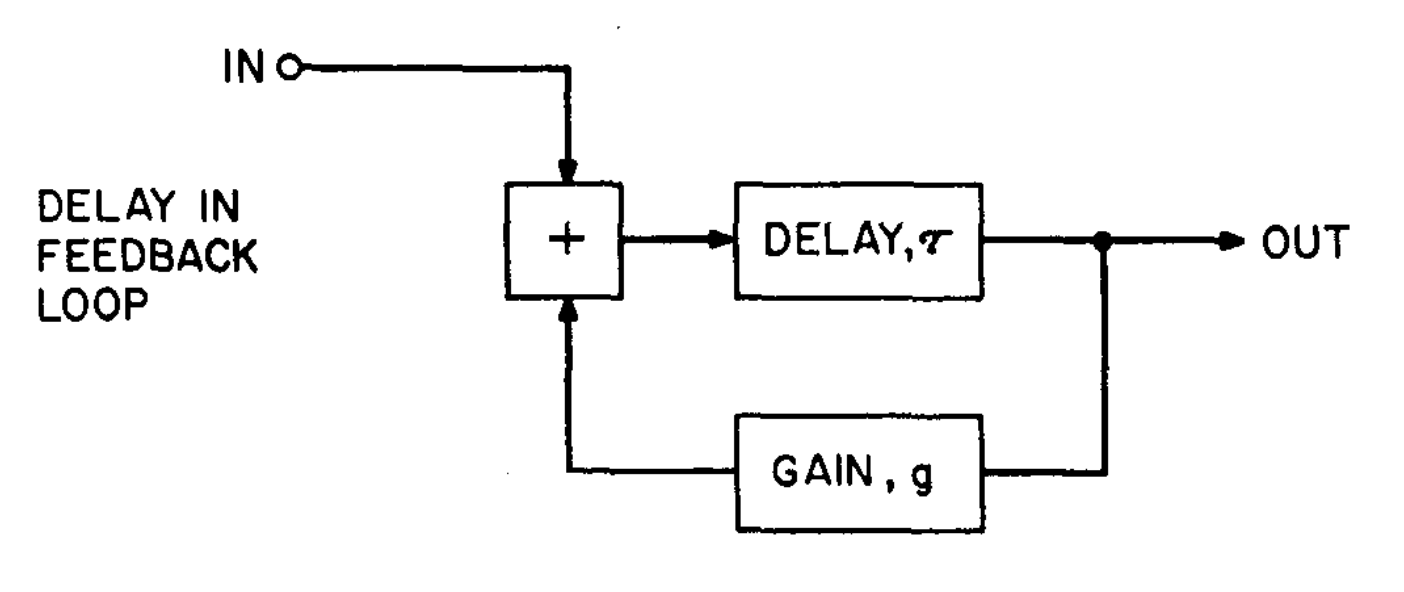
\includegraphics[width=\textwidth]{CAPITOLI/0500/IMG/dfl.png}
  \caption[]{Delay in Feedback Loop. Schroeder, 1962.}
  \label{schroeder:dfl}
\end{figure}

Il percorso di costruzione di un sistema di riverberazione in grado di dare
densità alle riflessioni e risposta timbrica a magnitudine lineare parte,per
\ms~dal più semplice filtro a struttura ricorsive \emph{IIR}. Il
cuore attorno a cui ruota la linea di retroazione è un ritardo variabile, che
cambia il comportamento temporale e quindi spettrale del filtro in funzione
dell'unità di ritardo.

\begin{figure}[t!]
  \centering
  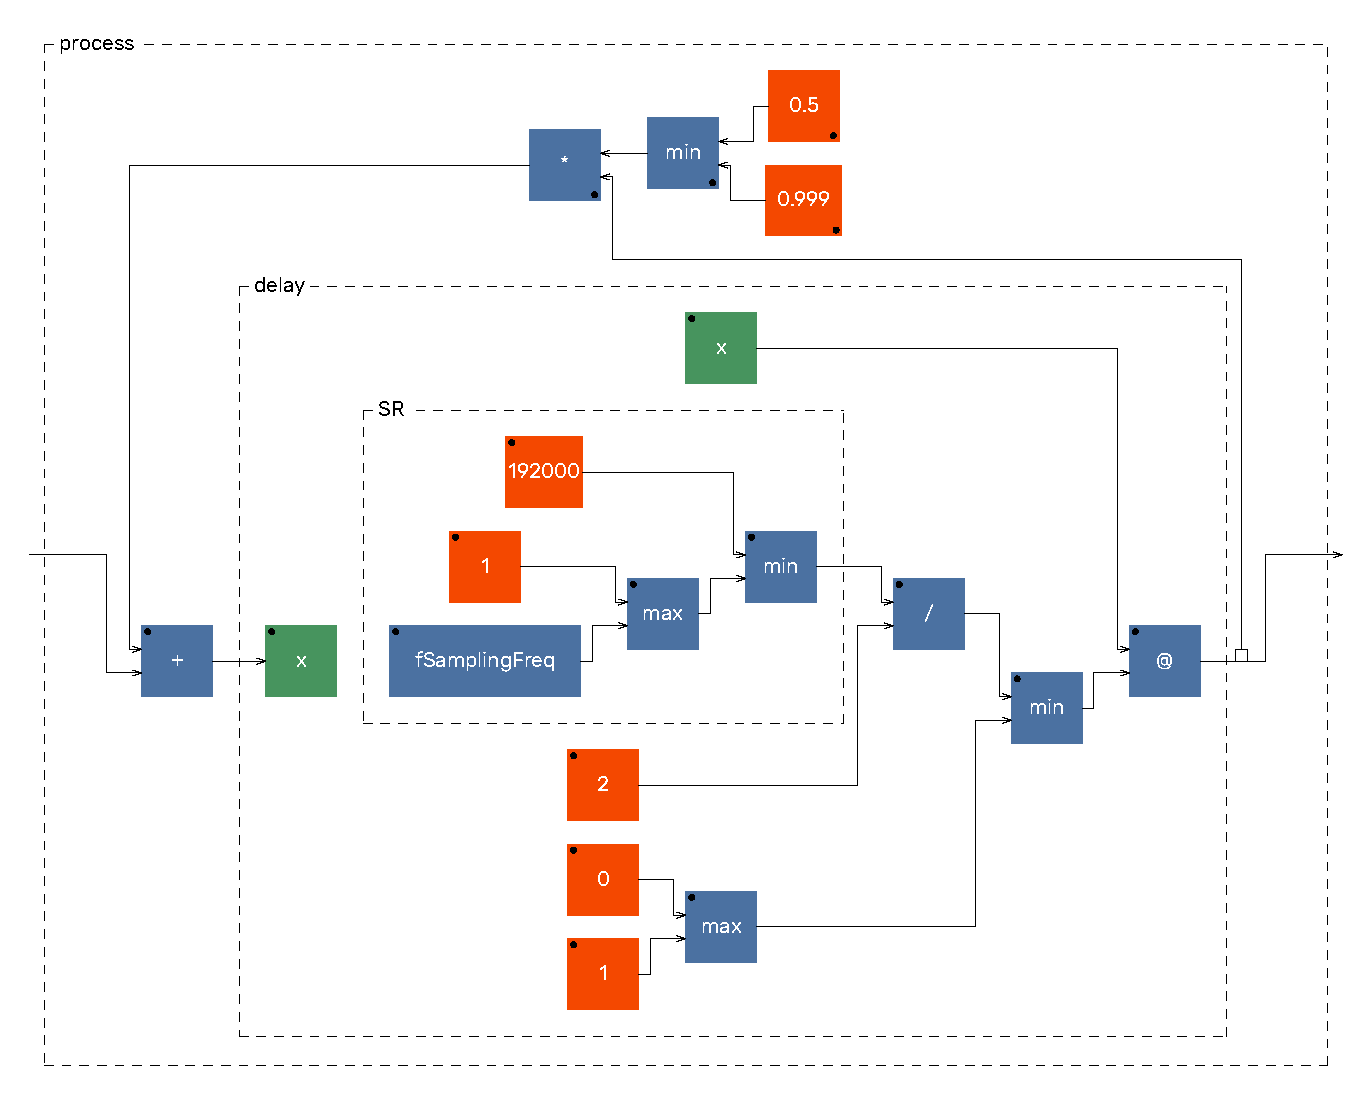
\includegraphics[width=\textwidth]{CAPITOLI/0500/CODES/REV/dfl-svg/process.pdf}
  \caption[]{Delay in Feedback Loop. Implementazione Faust.}
  \label{faust:dfl}
\end{figure}

La linea di ritardo alimentata da un circuito di retroazione controllato dal
coefficiente $g < 1$.  Il filtro prevede un valore di ritardo $t >= 1$ applicato a
tutti i campioni in entrata, situazione che può avere diversi significati,
come cercherò di spiegare in seguito.

Diagramma a blocchi sotto gli occhi (fig. \ref{schroeder:dfl}), il codice \faust
per la realizzazione di tale oggetto è il seguente.

\lstinputlisting{CAPITOLI/0500/CODES/REV/dfl.dsp}

Il codice può essere smontato e descritto in più parti per comprenderne la sintassi.

Il blocco di ritardo \texttt{delay} deve essere inizializzato con l'allocazione
di memoria massima in campioni. L'impostazione inserita \texttt{SR/2} permette
di avere almeno mezzo secondo a qualsiasi requenza di campionamento. Il tempo
$t$ di ritardo effettivo, in quanto unità al campione, deve essere necessariamente
un intero, motivo per cui la variabile in entrata $t$ viene passata per una
funzione \texttt{int} che ne scarta eventuali valori decimali.

L'uscita del blocco di ritardo viene prelevata prima dell'uscita dal filtro e
reindirizzata alla sua entrata, adeguatamente scalata dal coeffficiente $g < 1$,
in somma con l'entrata del filtro.

\begin{figure}[ht]
  \centering
  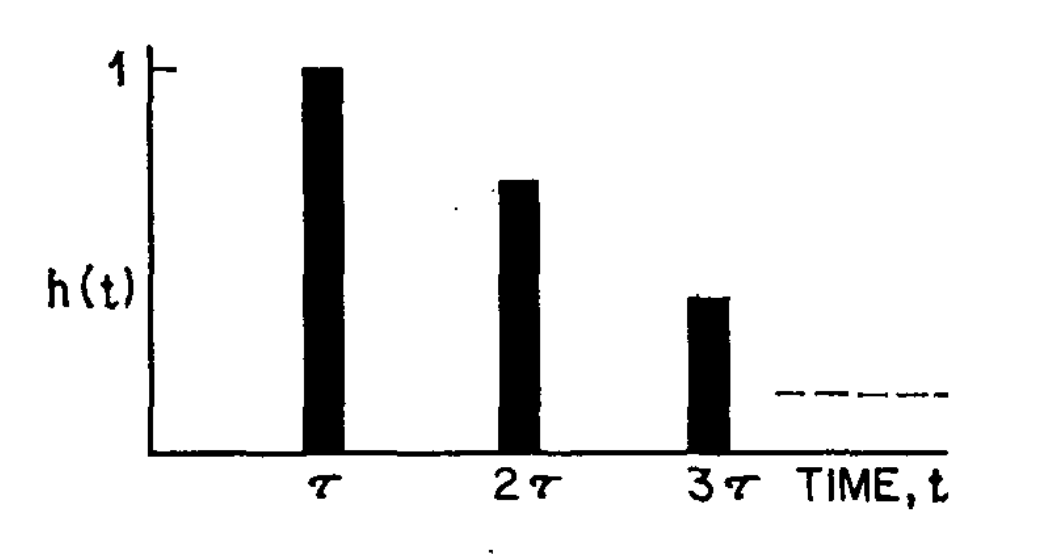
\includegraphics[width=\textwidth]{CAPITOLI/0500/IMG/dfl-ir.png}
  \caption[]{Schroeder dfl impulse response.}
  \label{schroeder:dflir}
\end{figure}

Schoreder fornisce una chiara descrizione del funzionamento temporale del filtro
ed attraverso un diagramma ne mostra la risposta all'impulso. La figura
\ref{schroeder:dflir} mostra il comportamento del filtro ad un tempo $t$
consistente in ripetizioni successive per multipli interi $2t$, $3t$ \ldots fino
al completo esaurimento dell'ampiezza per opera del coefficiente scalare $g$.

\begin{figure}[ht]
  \centering
  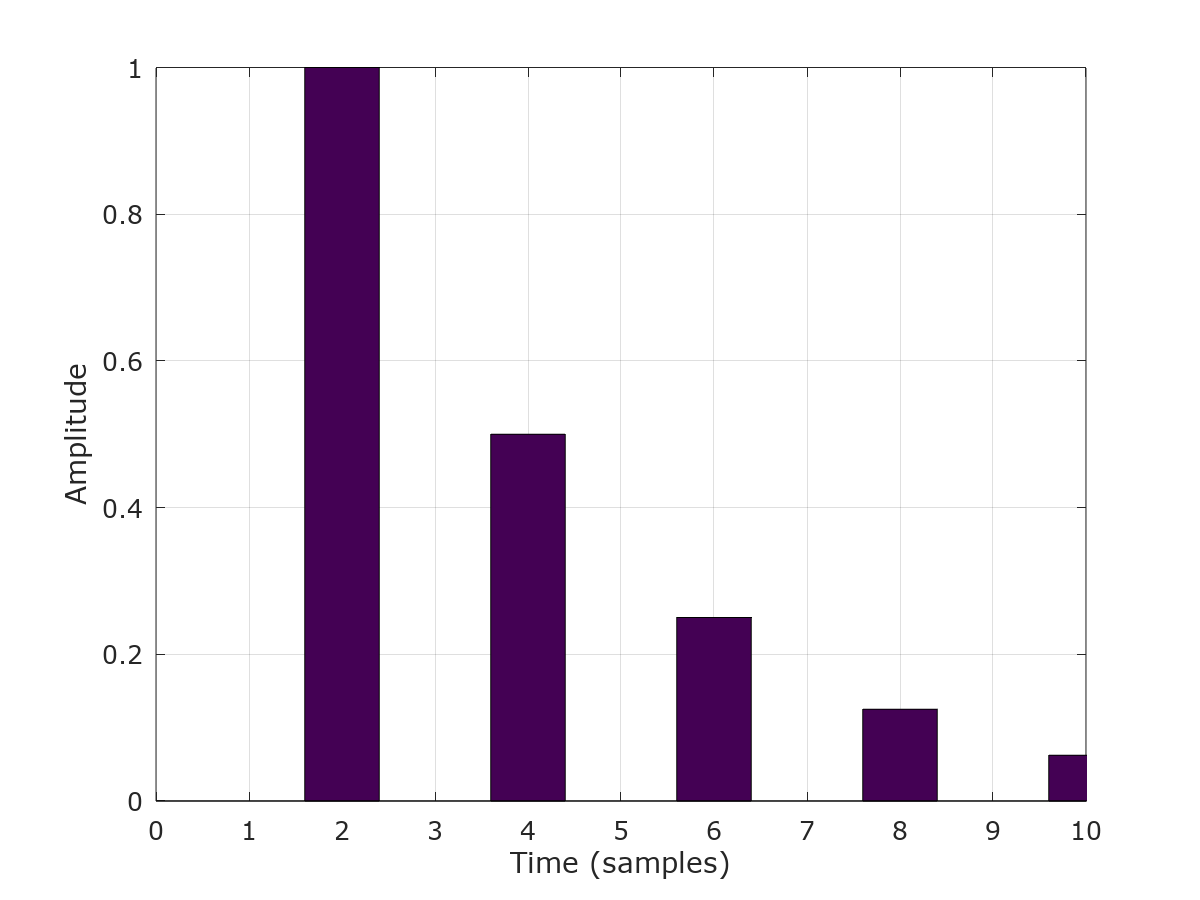
\includegraphics[width=\textwidth]{CAPITOLI/0500/CODES/REV/dfl.png}
  \caption[]{Faust dfl impulse response.}
  \label{faust:dflir}
\end{figure}

La risposta all'impulso illustrata in figura \ref{schroeder:dflir} indica un
decadimento esponenziale per ogni riflessione eco.

Possiamo descrivere allo stesso modo il nostro modello: il tempo di ritardo $t$
regola le nuove occorrenze dell'impulso generate dal circuito di retroazione
scalate dal coefficiente $g$. Pur avendo creato un modello di filtro
apparentemente identico, producente un diagramma a blocchi \ref{faust:dfl}
piuttosto fedele al modello di Schroeder, la risposta all'impulso del nostro
filtro si comporta in modo diverso, motivo per cui merita uno sguardo di analisi
e un'attenta riflessione.

La risposta all'impulso di figura \ref{faust:dflir} è stata generata impostando
le variabili $t=1$ (un campione di ritardo) e $g=0.5$ (ampiezza dimezzata ad
ogni giro di feedback). Ci si aspetta quindi un comportamento molto simile a
quello descritto da Schroeder, per una successione di multipli di $1$ dovremmo
avere il primo impulso nella posizione $n[1]$ con ampiezza $a=1$ (non scalata,
non l'impulso non è ancor transitato nel ciclo di ffeedback). Il secondo impulso
dovrebbe essere posizionato subito dopo il primo, nella posizione $n[2]$ con
ampiezza $a=0.5$, e cosi proseguendo. Tuttavia, osservando l'indicizzazione dei
campioni sull'asse delle ascisse della figura \ref{faust:dflir} si può constatare
che in realtà il nostro filtro sta impiegando due campioni per ogni ciclo
impulsivo in luogo di uno, posizionando gli impulsi per $2t$.

La motivazione di questa differenza è nascosta dietro al significato del diagramma
a blocchi di entrambe le rappresentazioni. Nella prima, quella originaria di Schroeder,
il punto di prelievo del segnale per il ciclo di feedback è a tempo zero, ovvero
linea che porta il segnale dall'uscita del blocco di ritardo all'entrata della
somma è istantanea. Nella descrizione algoritmica di faust mediante diagramma
a blocchi invece l'operatore $~$ produce contestualmente al prelievo del segnale,
un inevitabile campione di ritardo. La linea di ricircolo quindi, nel momento
in cui alimenta il blocco di ritardo, porta già un campione di ritardo su quello
corrente.

La correzione di questo filtro per ottenere il comportamento prospettato da Schroeder
consiste nel sottrarre il campione di ritardo, prodotto dalla ricorsione, alla
variabile $t$ con $t-1$. Questo tipo di intervento per $t=$ produrrà $t=1-1=0$
ovvero zero campioni di ritardo all'uscita, un campione, come richiesto,
scalato in $g$ all'entrata della somma di ricircolo. Questo tipo di operazione
crea però un offset temporale in quanto la sequenza di campioni ritardati, ora
corretta, si trova in uscita un campione prima (ritardo zero) di quello richiesto.
Anche questa problematica è risolvibile inserendo un ulteriore campione di ritardo
\texttt{mem} all'uscita dell'algoritmo, in modo da bilanciare l'intera sequenza
temporale.

\lstinputlisting{CAPITOLI/0500/CODES/REV/dflc.dsp}

La risposta all'impulso del filto corretto è ora coerente con le aspettative.

\begin{figure}[ht]
  \centering
  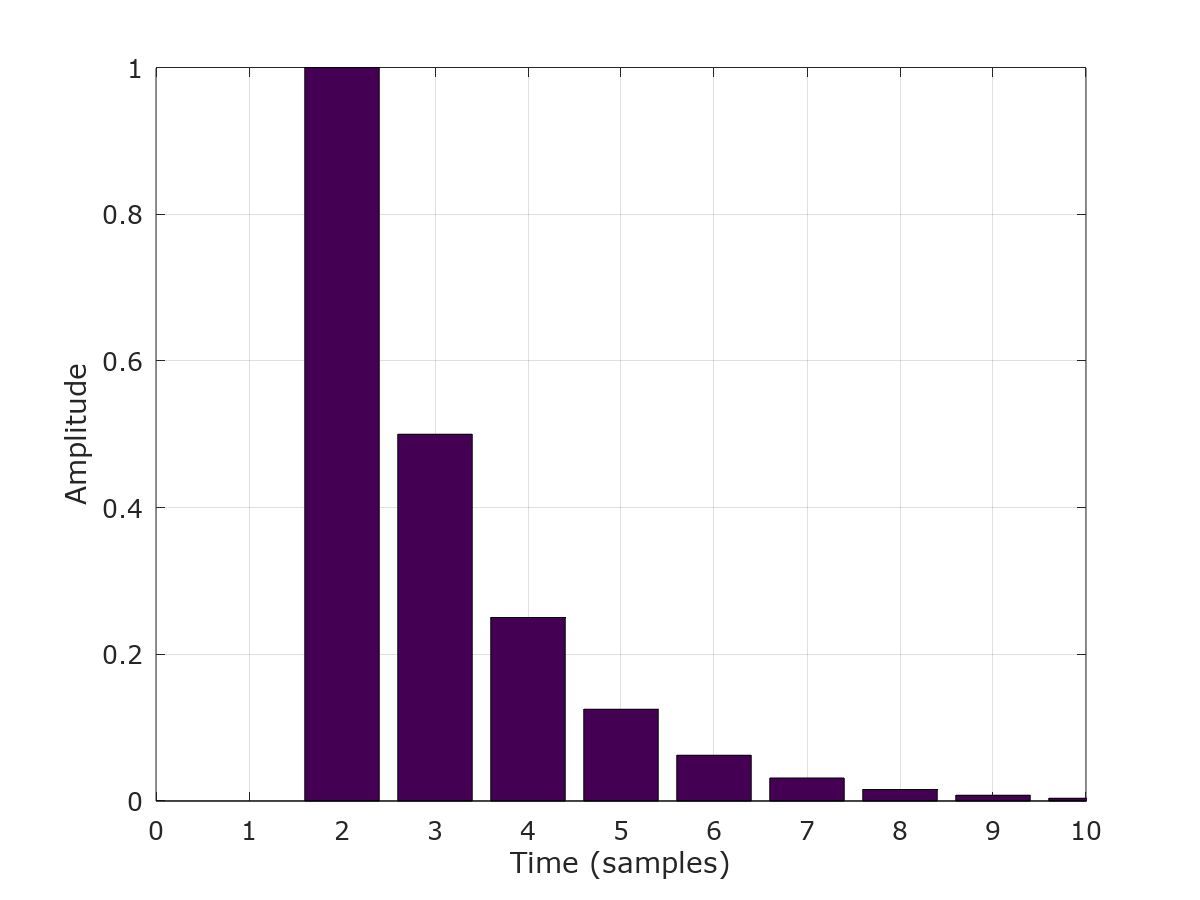
\includegraphics[width=\textwidth]{CAPITOLI/0500/CODES/REV/dflc.png}
  \caption[]{Faust dfl impulse response.}
  \label{faust:dflir}
\end{figure}

Il filtro appena costruito può operare tempi di ritardo tra $1$ e \emph{Nyquist}.
Questo comportamento può portare a diversi risultati sonori, dal più diretto
ritardo di una quantità di campioni indicata con $g=0$, oppure ad un filtraggio di componenti
spettrali in funzione di $t$ e $g$.

\begin{figure}[h]
  \centering
  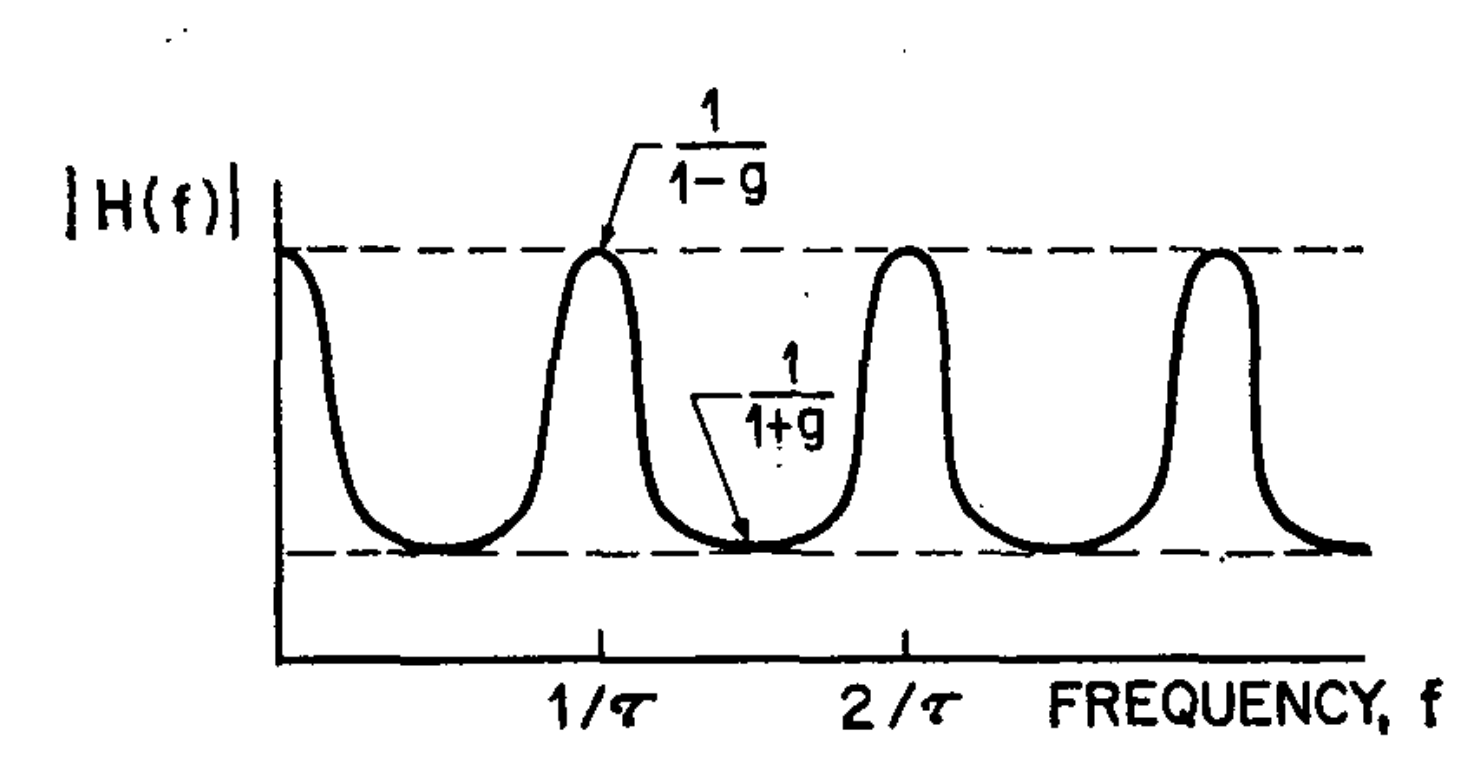
\includegraphics[width=\textwidth]{CAPITOLI/0500/IMG/dfl-fr.png}
  \caption[]{Schroeder dfl risposta in requenza, \emph{”somigliante ad un pettine”}.}
  \label{schroeder:dflffr}
\end{figure}

\begin{quote}
  The amplitude-frequency responce has the appearance of a comb with periodic
  maxima and minima\ldots It is these peaks and valleyys which impart the undesidered
  “colored” qualityy to sound reverberated by devices like that.
\end{quote}

Il rapporto tra la risposta massima e quella minima è espresso dalla formula:

\begin{equation}
  \label{comb-filter}
  H_{max}/H_{min} = (1+g)/(1-g)
\end{equation}

il che porta a considerare che per un coefficiente $g=0.708$ corrispondente ad
un abbattimento di $-3dB$ il rapporto di di $5.849:1$ (espresso da $1.708/0.292$)

\begin{equation}
  \label{hmax}
  \Delta_{amp} = 20\times Log_10(5.849) = 15.34 dB
\end{equation}

ovvero $15.34dB$ di escursione.

\begin{quote}
  In a search for better artificial reverberators\ldots (we) noted that certain
  mixture of the output of the multiply delayed sound and the undelayed sound
  would result in an equal response of the reverberator for all frequencies.
\end{quote}

Questo passo è cruciale per comprendere il processo evolutivo dei meccanismi
riverberanti di Schroeder. Il filtro IIR passa da un campione di ritardo (passa
basso) ad un delay variabile (comb-filter) e sta per diventare un filtro
lineare in frequenza (all-pass) attraverso una oculata gestione dei rapporto tra
suono diretto e suono ritardato. La proporzione per contenere l'energia unitaria
su tutto lo spettro di frequenze è $-g$ per il segnale diretto e $1-g^2$
per il segnale ritardato.

\begin{figure}[ht]
  \centering
  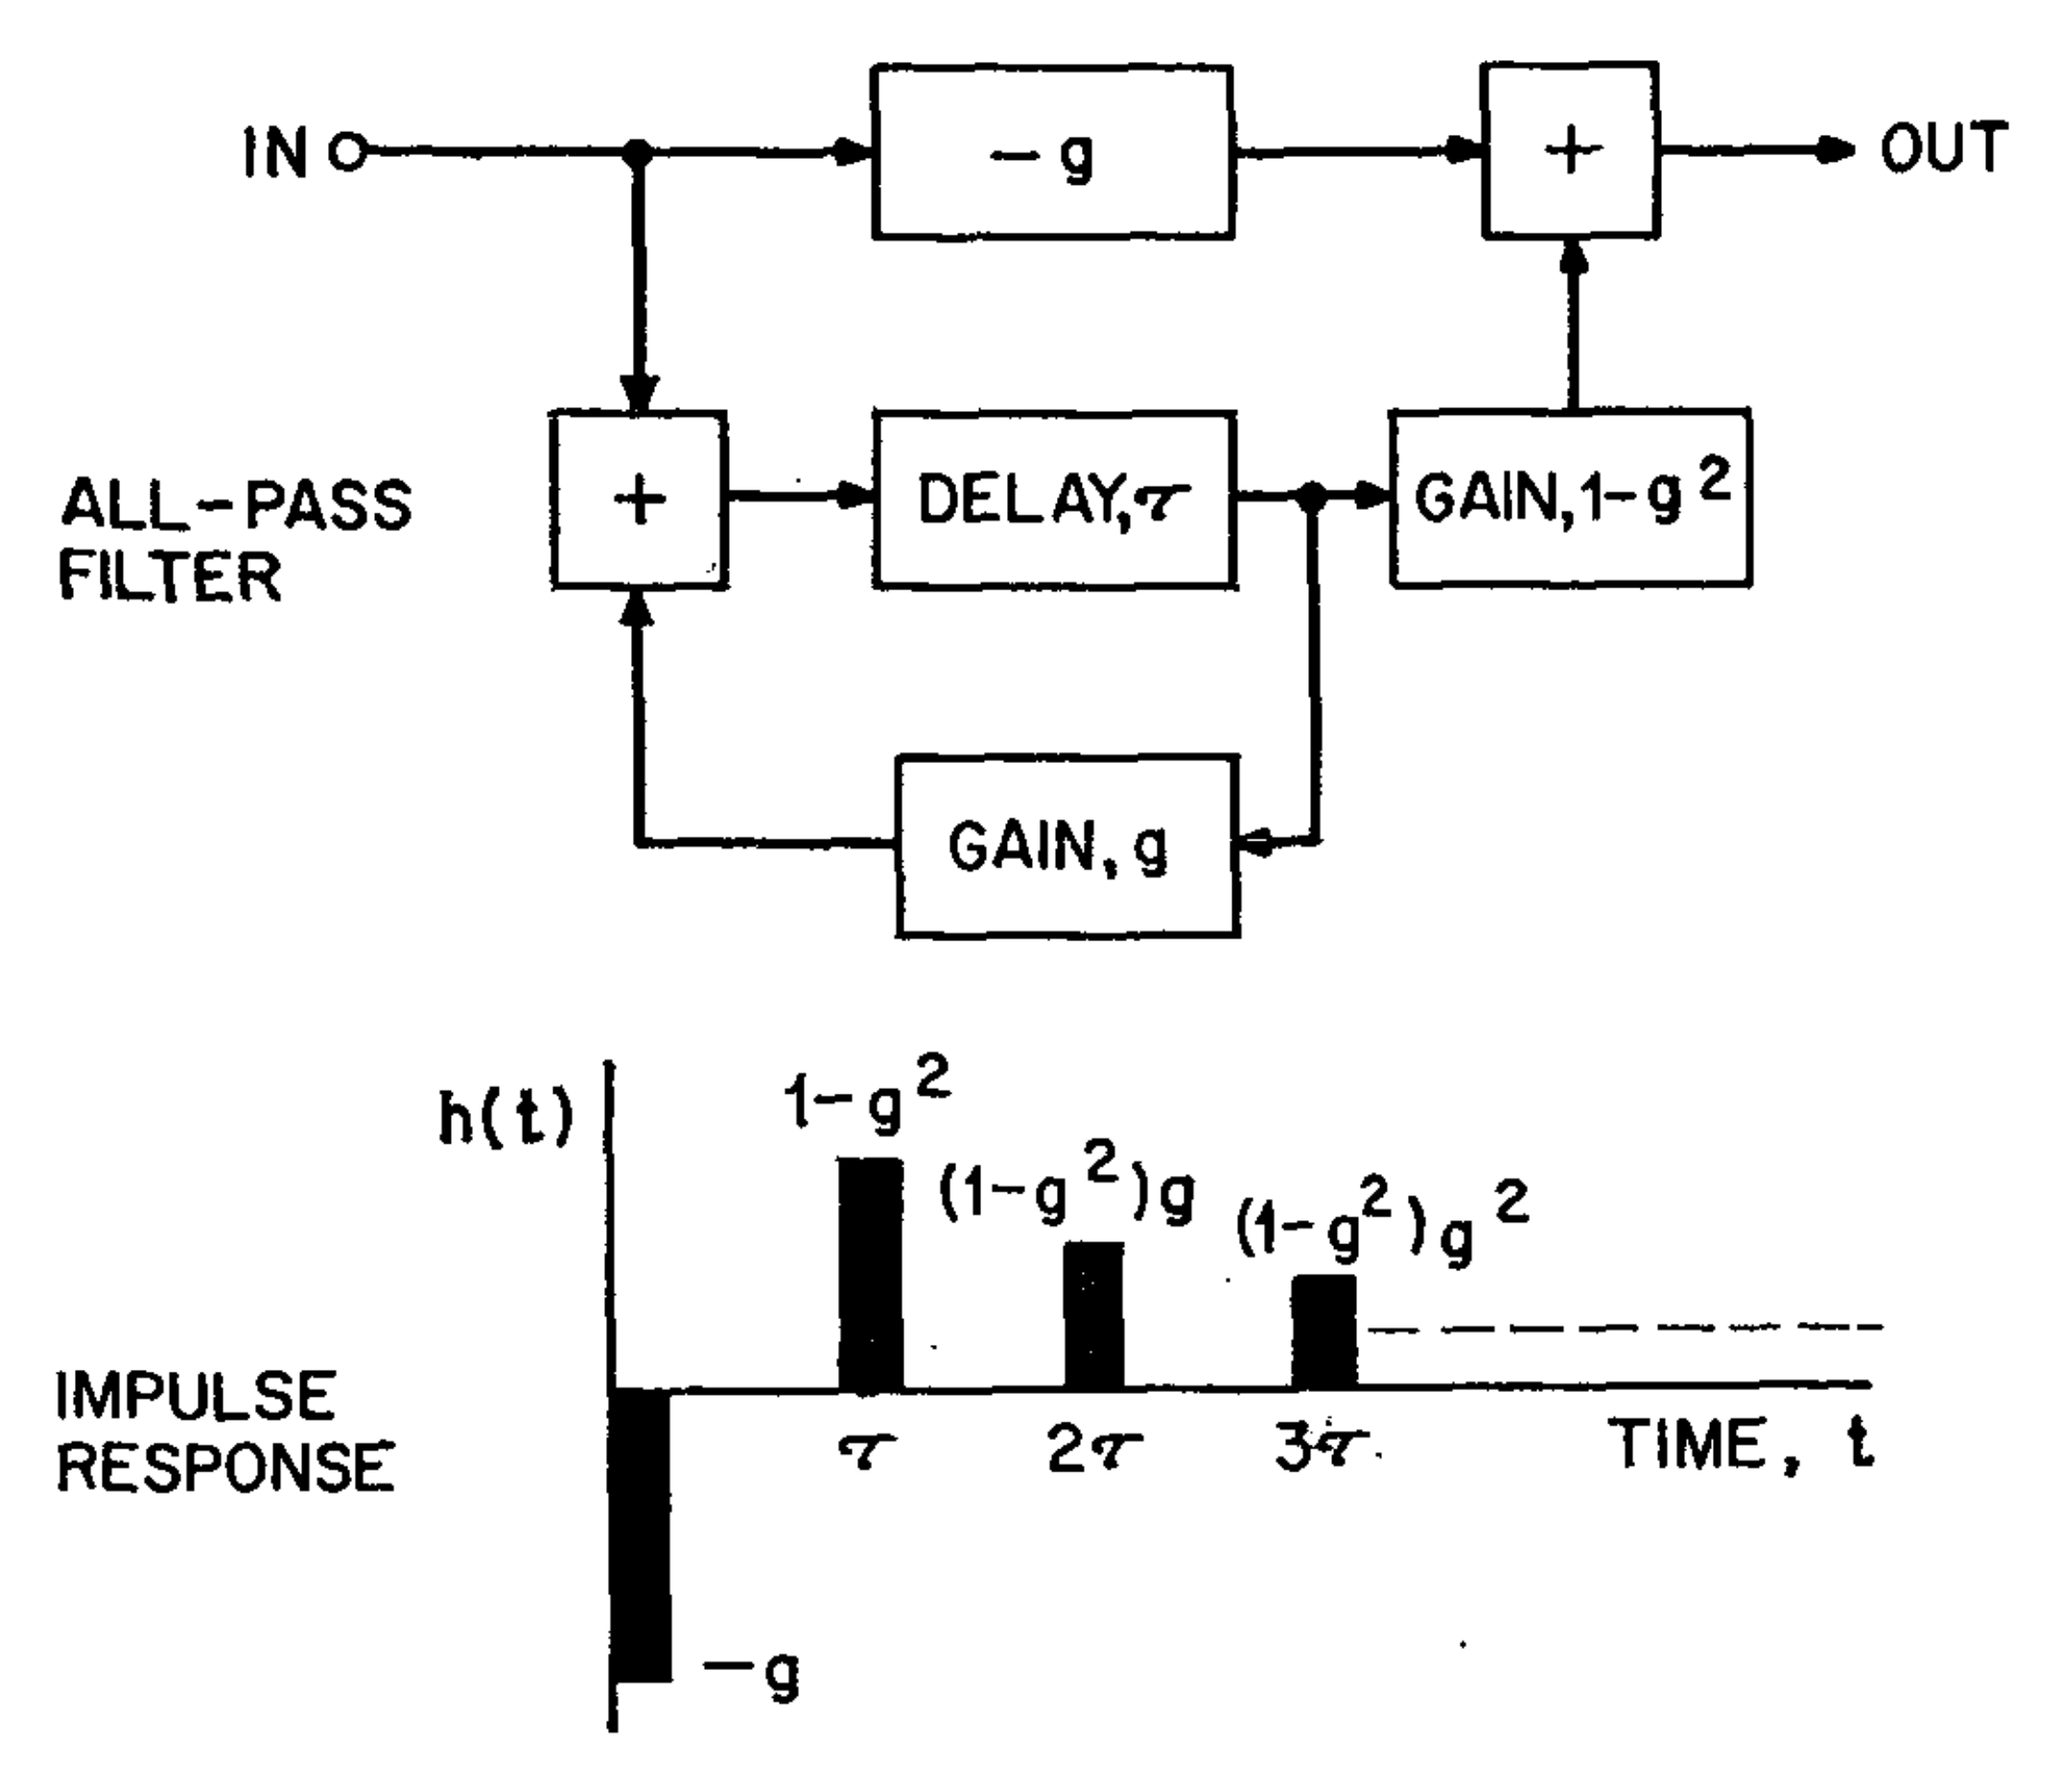
\includegraphics[width=\textwidth]{CAPITOLI/0500/IMG/allpass.png}
  \caption[]{All-pass, diagramma a blocchi e risposta all'impulso.}
  \label{schroeder:allpass}
\end{figure}

\begin{quote}
  \ldots the addition of a suitably proportioned uunudelayyed path has converted
  the comb-filter (fig. \ref{schroeder:dfl}) into an all-pass (fig.
  \ref{schroeder:allpass}). This is not a mere academic result.
\end{quote}

Il filtro all-pass ora permette di passare tutte le frequenze con eguale ampiezza
e senza “colorare” il segnale. Si possono connettere tra loro diverse unità di
questo tipo per raggiungere la densità di eco necessaria. Inoltre il filtro
all-pass condivide con i filtri comb le proprietà del feedback e del decadimento
esponenziale dell'energia, lo stesso comportamento che si presenta nelle buone
situazioni acustiche.

\lstinputlisting{CAPITOLI/0500/CODES/REV/apf.dsp}

\subsection{Synthetic Stereo Reverberation}

Nel 1971 \mg~pubblica per \emph{Studio Sound} \ref{} 




\printbibliography
\end{refsection}
